\begin{figure}[h] % h means place here if possible
\centering
\def\layersep{2.5cm}
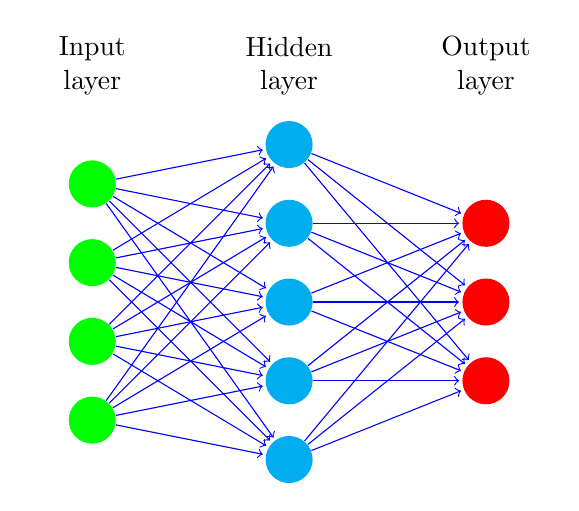
\begin{tikzpicture}[shorten >=1pt,->,draw=blue, node distance=\layersep]
    \tikzstyle{every pin edge}=[<-,shorten <=1pt]
    \tikzstyle{neuron}=[circle,fill=black!25,minimum size=17pt,inner sep=0pt]
    \tikzstyle{input neuron}=[neuron, fill=green];
    \tikzstyle{output neuron}=[neuron, fill=red];
    \tikzstyle{hidden neuron}=[neuron, fill=cyan];
    \tikzstyle{annot} = [text width=4em, text centered]

    \node[input neuron] (I-1) at (0,-1) {}; % {$T_{2m}$};
    \node[input neuron] (I-2) at (0,-2) {}; % {$q_v$};
    \node[input neuron] (I-3) at (0,-3) {}; % {$RH$};
    \node[input neuron] (I-4) at (0,-4) {}; % {$p_s$};

    % Draw the input layer nodes
    %\foreach \name / \y in {1,...,4}
    % This is the same as writing \foreach \name / \y in {1/1,2/2,3/3,4/4}
    %    \node[input neuron, pin=left:Input \#\y] (I-\name) at (0,-\y) {};

    % Draw the hidden layer nodes
    \foreach \name / \y in {1,...,5}
        \path[yshift=0.5cm]
            node[hidden neuron] (H-\name) at (\layersep,-\y cm) {};

    % Draw the output layer node
    \node[output neuron, right of=H-2] (O) {};
    \node[output neuron, right of=H-3] (O1) {};
    \node[output neuron, right of=H-4] (O2) {};


    % Connect every node in the input layer with every node in the
    % hidden layer.
    \foreach \source in {1,...,4}
        \foreach \dest in {1,...,5}
            \path (I-\source) edge (H-\dest);

    % Connect every node in the hidden layer with the output layer
    \foreach \source in {1,...,5}
        \path (H-\source) edge (O);
        %\path (H-\source) edge (o1);
        %\path (H-\source) edge (o2);

    % Does the same thing the loop does had to do it manually tho
    \path (H-1) edge (O1);
    \path (H-2) edge (O1);
    \path (H-3) edge (O1);
    \path (H-4) edge (O1);
    \path (H-5) edge (O1);
    
    \path (H-1) edge (O2);
    \path (H-2) edge (O2);
    \path (H-3) edge (O2);
    \path (H-4) edge (O2);
    \path (H-5) edge (O2);

    % Annotate the layers
    \node[annot,above of=H-1, node distance=1cm] (hl) {Hidden layer};
    \node[annot,left of=hl] {Input layer};
    \node[annot,right of=hl] {Output layer};
\end{tikzpicture}
\caption{Fully connected feed forward neural network with one hidden layer. The connections between the layers are the weights. The sketch is based on the example \citepaper{ffnn}.}
\label{fig:one_layer_mlp}
\end{figure}
%The input layer has four units, the hidden layer has five and the output layer has three. In total there are 35 parameters in this network (37 if bias is included).